\chapter{Floppy Disks And D81 Images}
\label{cha:freezer}

\phantomsection

\section{Terminology}
Before you get to know how to use the various disk drives that work with the MEGA65, it's important to be aware
of some specific terminology which CBM computers and the MEGA65 uses. This includes {\bf BASIC} and {\bf CBDOS},
which use the following:

{\bf UNIT} is a device number in the range of 0-31.
The numbers from 0 to 11 are reserved for following device types:

\setlength{\tabcolsep}{1mm}
\begin{center}
\begin{tabular}{|l|l|l|}
\hline
{\bf Unit} \# & {\bf Device}  & {\bf Comment} \\
\hline
0        & KEYBOARD & Input \\
1        & unused   & Was used for TAPE on the C64 \\
2        & unused   & Was used for RS232 on the C64 \\
3        & SCREEN   & Input/Output     \\
4-5      & IEC PRINTER  & Output     \\
6-7      & IEC PLOTTER  & Output     \\
8-9      & CBDOS drives & Floppy drive or disk image \\
10-11    & IEC drives   & 1541, 1571, 1581, FD-2000 \\
\hline
\end{tabular}
\end{center}

{\bf DRIVE} is the drive number inside a {\bf UNIT}:

\setlength{\tabcolsep}{1mm}
\begin{center}
\begin{tabular}{|l|l|l|}
\hline
{\bf Device}  & {\bf Drive Numbers} & {\bf Comment} \\
\hline
1541 IEC & 0             & Single drive \\
1571 IEC & 0             & Single drive \\
1581 IEC & 0             & Single drive \\
FD-2000 IEC & 0             & Single drive (CMD)\\
FD-4000 IEC & 0             & Single drive (CMD)\\
SD2IEC      & 0             & Drive images\\
4040 IEEE-488 & 0,1             & Dual drive (CMD)\\
8050 IEEE-488 & 0,1             & Dual drive (CMD)\\
8250 IEEE-488 & 0,1             & Dual drive (CMD)\\
\hline
\end{tabular}
\end{center}

For all single drives the drive number is always 0.
These are all known drives with an IEC interface. For example
the CBM drives 1541, 1571, 1581, the CMD drives FD-2000 and FD-4000, as well as
SD2IEC devices, which emulate a CBM drive using disk images on SD card.

Dual disk drives such as the 4040, 8050, and 8250 (which use drive numbers
0 and 1) are equipped with an IEEE-488 interface, and need
an IEEE-488 to IEC converter to be used on the MEGA65.

The internal floppy controller of the MEGA65 can control
two floppy drives (one internal and one external, both of which must be attached to the same
ribbon cable). The {\bf FREEZER} can be used to assign D81 images from an
SD card to the drive numbers 0 and/or 1, instead of physical floppy drives.

{\bf BASIC} commands that address files or disks include
{\bf U} for UNIT and {\bf D} for drive.
The default settings are {\bf UNIT = 8} and {\bf DRIVE = 0}.

\section{The Freezer}
The {\bf FREEZER} is a tool for changing system parameters at any time
regardless of the currently running program. The {\bf FREEZER} is invoked
by pressing \widekey{RESTORE} for approximately half to one second.
The current status of the computer is frozen and the freezer menu,
similar to the picture below is displayed.
Most options are self explaining or will be covered in detail in the
online documentation. This chapter describes, how to assign disk images
and the internal floppy disk drive.

\begin{center}
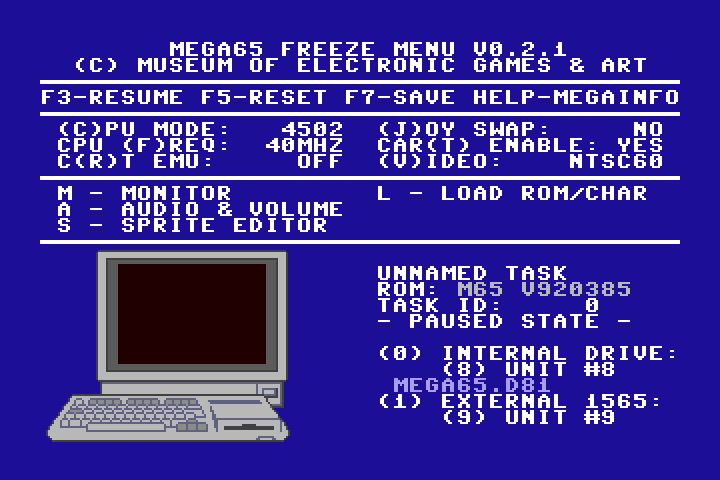
\includegraphics[trim= 10mm 20mm 10mm 20mm,clip,width=0.7\linewidth]{images/freezer.jpg}
\end{center}

The bottom/right region of the freezer screen shows the current assignments.
The internal CBDOS (Computer Based Disk Operating System) can handle two
3.5" disk drives or D81 images.
Drive 0 can be assigned to the internal floppy disk drive or a D81 disk image,
whereas Drive 1 can be assigned to an external floppy disk drive (connected to the
same ribbon cable as the internal drive) or a D81 disk image.

The typical configurations are usually one of the following:
\begin{center}
\begin{tabular}{|l|l|l|}
\hline
{\bf Drive 0 Assignment} & {\bf Drive 1 Assignment} \\
\hline
Internal floppy disk drive &  Disk image \\
Disk image                 &  Disk image \\
\hline
\end{tabular}
\end{center}

The assignment, and the mounting of disk images can be done by pressing
\megakey{0} for drive 0 or \megakey{1} for drive 1.

The drive numbers are used internally by CBDOS. However, {\bf BASIC} and Kernal
address the storage devices by {\bf UNIT} numbers.
CBDOS fakes two single drives for the
operating system, by assigning separate unit numbers to drive 0 and drive 1.
The default assignment is:

\begin{center}
\begin{tabular}{|l|l|l|}
\hline
{\bf Unit/Drive} & {\bf Assignment} \\
\hline
UNIT 8, DRIVE 0  & Internal drive 0 (internal floppy or disk image) \\
UNIT 9, DRIVE 0} & Internal drive 1 (external floppy or disk image) \\
\hline
\end{tabular}
\end{center}


You may wish to change this unit assignment, if for example
a 1541 drive is plugged in as unit 8 to the IEC port.
In this case, the internal drive assignment can be switched to an alternative unit,
to avoid conflict.

\megakey{8} toggles the unit assignment of drive 0 between 8 and 10. \\
\megakey{9} toggles the unit assignment of drive 1 between 9 and 11.

After setting the preferences, the {\bf freezer} can be exited
with \megakey{F3}. The {\bf freezer} restores the screen and
returns to the interrupted program.

The drive and unit assignments are temporary and will be reset to default
after power down or reset. For permanent settings use the {\bf CONFIGURE}
menu.

